% Tipo de documento
\documentclass[12pt, twoside, a4paper, openany, bibliography=totoc, numbers=noenddot]{scrbook}

% Añadir caracteres no anglosajones como tildes, ñ, ¿, ¡, etc.
\usepackage[utf8]{inputenc}
\usepackage[spanish]{babel}
 
% Añadir gráficos
\usepackage{graphicx}
% Carpeta donde se encuentran las imágenes
\graphicspath{ {figs/} }
\usepackage[labelfont=bf]{caption}
\usepackage{subcaption}
\DeclareGraphicsExtensions{.pdf,.png,.jpg}
\usepackage{chngcntr}
\counterwithout{figure}{chapter}

% Listas con corchetes tipo [1], [2]...
\usepackage{enumitem}

% Permite usar hipervínculos
\usepackage[hidelinks]{hyperref}

\usepackage{afterpage}

\newcommand\blankpage{
    \null
    \thispagestyle{empty}
    \newpage}

% Floating options
\usepackage{float}
\restylefloat{figure}

% Márgenes
\usepackage[left=2.5cm,right=2.5cm,bindingoffset=0.5cm]{geometry}
\setlength{\headheight}{20pt}

% Estilo de los titulos de los capítulos
\usepackage{titlesec}
\titleformat{\chapter}[display]
{\normalfont\huge\bfseries}{\chaptertitlename\ \thechapter}{20pt}{\Huge}[\vspace{2ex}\titlerule]

% Fuente utilizada para el cuerpo
\usepackage[bitstream-charter]{mathdesign}

% Permite usar frames (cajas)
\usepackage{framed}

% Permite usar colores
\usepackage[usenames,dvipsnames,svgnames,table]{xcolor}

% Permite el uso de cabeceras y pies de página
\usepackage{fancyhdr}

% Biblatex
\usepackage[backend=bibtex,style=numeric,natbib=true]{biblatex}
\addbibresource{bibliography.bib}

% Permite realizar rotaciones
\usepackage{rotating}

% Opciones de tablas
% Para crear líneas más gruesas
\usepackage{tabu}
\counterwithout{table}{chapter}

\captionsetup[figure]{font=bf,position=below}

% Prevents placing floats before the section 
\usepackage{placeins}
\makeatletter
\AtBeginDocument{%
  \expandafter\renewcommand\expandafter\subsection\expandafter
    {\expandafter\@fb@secFB\subsection}%
  \newcommand\@fb@secFB{\FloatBarrier
    \gdef\@fb@afterHHook{\@fb@topbarrier \gdef\@fb@afterHHook{}}}%
  \g@addto@macro\@afterheading{\@fb@afterHHook}%
  \gdef\@fb@afterHHook{}%
}
\makeatother

\PassOptionsToPackage{usenames,dvipsnames}{xcolor}

\usepackage[usenames,dvipsnames]{xcolor}
\usepackage[draft]{pgf}
\usepackage{listings}
\usepackage[svgnames]{xcolor}

% Bordes en imágenes
\usepackage[export]{adjustbox}

% Múltiples líneas en una misma celda de una tabla => \specialcell{}
\newcommand{\specialcell}[2][c]{%
  \begin{tabular}[#1]{@{}c@{}}#2\end{tabular}}

\lstset{
     language        = php,
     basicstyle      = \small\ttfamily,
     keywordstyle    = \color{blue},
     stringstyle     = \color{red},
     identifierstyle = \color{ForestGreen},
     commentstyle    = \color{gray},
     emph            =[1]{php},
     emphstyle       =[1]\color{black},
     emph            =[2]{if,and,or,else},
     showstringspaces=false,
     emphstyle       =[2]\color{yellow},
     backgroundcolor=\color{gray!10},
     breaklines=true,
     numbers=left,
     numberstyle=\footnotesize,
     showspaces = false,
     showstringspaces = false,
     tabsize = 2,
     %numbers=left,
     %numbersyle=\tiny
     frame=single,
     xleftmargin=5pt,
     xrightmargin=3pt,
     aboveskip = 20pt,
     rulecolor=\color{black},
     escapechar=|
}
     
\renewcommand{\lstlistingname}{Código}
\DeclareCaptionFormat{listing}{\rule{\dimexpr\textwidth\relax}{0.4pt}\par\vskip1pt#1#2#3}
\captionsetup[lstlisting]{format=listing,singlelinecheck=false, margin=0pt, font={sf},labelsep=space,labelfont=bf}

\begin{document}

\fancyhead[R]{\slshape \rightmark}
\fancyfoot[C]{\thepage}

% Permite escoger la profundidad de las secciones (1.1, 1.1.1.2...)
\setcounter{secnumdepth}{2}

%----------------------------------------------------%
%                      PORTADA                       %
%----------------------------------------------------%

\pagestyle{empty}

% Define una línea horizontal para el título
\newcommand{\HRule}{\rule{\linewidth}{0.5mm}} 

% Centra el contenido
\begin{center}
	% Título entre dos líneas horizontales
	\HRule \\[0.5cm]
	\vspace{0.5cm}
	\textbf {
		{\huge V de Big Data}\\
		\vspace{0.3 cm}
		Revolucionando el procesamiento de datos masivos\\
	}
	\vspace{0.5cm}
	\HRule \\[0.5cm]
	{\large
		
		\vspace{1 cm}
		Máster en Sistemas Informáticos Avanzados\\
		Junio de 2017\\
		\vspace{3.0 cm}
		Autor:\\
		\vspace{0.2 cm}
		Xabier Zabala Barandiaran\\
		\vspace{1.0 cm}
		Supervisores:\\
		\vspace{0.2 cm}
		German Rigau i Claramunt\\
		{\small UPV/EHU\\}
		Iñigo Etxabe\\
		{\small Datik Información Inteligente S.L.\\}
	}

	\vspace{2.0 cm} 
	\begin{figure}[h!]
		\centering
		
\includegraphics[width=0.4\textwidth]{Ilustraciones/ehu.png}\hfill
		
\includegraphics[width=0.4\textwidth]{Ilustraciones/informatica.png}\hfill

	\end{figure}
\end{center}
\frontmatter
\pagestyle{plain}
\cleardoublepage

%----------------------------------------------------%
%                  AGRADECIMIENTOS                   %
%----------------------------------------------------%

\begin{flushright}
	\Large\textit{Agradecimientos}
\end{flushright}

En primer lugar, quisiera expresar mi gratitud a las personas que han posibilitado la concepción y el desarrollo de la presente tesina. Agradezco a German Rigau i Claramunt, supervisor del proyecto por parte de la UPV/EHU, la predisposición mostrada y el asesoramiento ofrecido durante el transcurso del mismo. Doy también las gracias a Inigo Etxabe y Beñat Aranburu, supervisores del proyecto por parte de Datik Información Inteligente, por poner a mi disposición todos los medios tecnológicos necesarios para llevar a cabo el trabajo y por el trato ofrecido desde el primer día.\\

Agradecer, cómo no, a mis padres José Javier Zabala y María Pilar Barandiaran el esfuerzo desempeñado para facilitarme, en la medida que les ha sido posible, el camino que he recorrido hasta llegar aquí. Me congratula haber sabido responder satisfactoriamente a la confianza que ellos han depositado en mí. Por todo lo que han hecho y por todo lo que suponen para mí, un beso enorme para los dos.\\

No quisiera olvidar aquellas personas que me han acompañado durante este maravilloso periplo. Doy las gracias a la cuadrilla y a la gente que he tenido la fortuna de conocer durante estos últimos años en la facultad. Quisiera agradecer especialmente a las personas que en este pasado lustro se han ganado a pulso el privilegio a ser parte importante de lo que me resta de existencia, a los cuales me atreveré a mencionar aún con el temor de dejar a alguna en el tintero: Adrián Núñez, Eider Irigoyen, Goiatz Irazabal, Jaime Altuna, Marta García y Mikel Etxeberria. No hallo palabras para expresar todo lo que os debo.\\

Por último, pero no por ello menos importante, quisiera evocar a todos los docentes que han tomado parte en mi formación desde aquel Septiembre del 2009 y agradecer a todos ellos el conocimiento compartido y el esfuerzo invertido en mí durante estos años.\\

Gracias de todo corazón a la gente mencionada en este breve capítulo por haber hecho de mí un mejor profesional y sobre todo una mejor persona, además de darme las fuerzas necesarias para seguir mejorando en ambos aspectos.\\


\cleardoublepage

%----------------------------------------------------%
%                      RESUMEN                       %
%----------------------------------------------------%

\section*{Resumen}

Proyecto Final del Máster en Sistemas Informáticos Avanzados. Estudio empírico sobre el rendimiento ofrecido por varias tecnologías emergentes en el campo del Big Data en comparación a una base de datos tradicional a la hora de operar en escenarios que requieren un almacenamiento y procesamiento eficaz de volúmenes masivos de datos.\\

Dos entornos de pruebas totalmente aislados han sido erigidos sobre la misma máquina física. En el primero, se ha construido un clúster compuesto por tres nodos virtuales que operan en la misma red privada. Dichos nodos han sido dotados de tecnología necesaria para el correcto funcionamiento de Apache Cassandra \cite{lakshman2010cassandra} y Apache Spark \cite{zaharia2010spark}. Sobre el segundo entorno, constituido por un nodo virtual de potencia equivalente al clúster ya mencionado, se ha instalado una instancia de MySQL Server. Una vez habiendo diseñado un conjunto de consultas equivalentes para ambas bases de datos, se ha procedido a poblar dichos sistemas de almacenamiento utilizando un data-set público de aproximadamente 25GB. Para finalizar, las consultas predefinidas han sido ejecutadas para así poder cuantificar el tiempo de respuesta ofrecido por cada entorno.\\

El estudio evidencia que a la hora de trabajar con volúmenes masivos de datos el binomio formado por Apache Cassandra y Apache Spark, además de ofrecer una solución totalmente escalable y tolerante a fallos, mejora sustancialmente el rendimiento ofrecido por MySQL Server. No obstante, para gozar de dichas ventajas, se antoja necesario invertir más tiempo en analizar exhaustivamente la naturaleza de los datos que se desean tratar.\\


Palabras Clave: Apache Cassandra, Apache Spark, Benchmark, Big Data, MySQL Server.\\

\cleardoublepage

%----------------------------------------------------%
%                    INDICE GENERAL                  %
%----------------------------------------------------%

\tableofcontents
\newpage

%----------------------------------------------------%
%                    INDICE FIGURAS                  %
%----------------------------------------------------%

\listoffigures
\newpage

%----------------------------------------------------%
%                    INDICE TABLAS                   %
%----------------------------------------------------%

\listoftables
\cleardoublepage

%----------------------------------------------------%
%                    INTRODUCCION                    %
%----------------------------------------------------%

\mainmatter
\fancyhead[LE,RO]{\itshape \nouppercase \rightmark}
\fancyhead[LO,RE]{\itshape \nouppercase Capítulo \arabic{chapter}}

%----------------------------------------------------%
%                    INTRODUCCION                    %
%----------------------------------------------------%

\pagestyle{fancy}

\chapter{Introducción}
\label{introduccion}

Desde Aristóteles y su libro Segundos Analíticos \footnote{\href{https://docs.google.com/a/datik.es/file/d/0By4kcbi6MzzdUHhVQnUtcTNUdk0/view}{Órganon II de Aristóteles: Segundo Analíticos se encuentra recopilado en él}} hasta Galileo, padre de la ciencia moderna, adalides del conocimiento han proclamado que un método de investigación basado en lo empírico y en la medición, sujeto a los principios específicos de las pruebas de razonamiento es el camino para conocer la verdad.\\

Hoy en día, época en la que los avances tecnológico han posibilitado observar y medir de forma exhaustiva un gran abanico de fenómenos, la ingente cantidad de datos que se genera en el proceso es, a veces, intratable por medio de las tecnologías convencionales, y por ende, es imposible extraer conocimiento. El problema, lejos de atenuarse, se acrecienta con el paso del tiempo, ya que, estudios como el realizado por McKinsey Global Institute estiman que el volumen de datos que se genera crece un 40\% cada año y auguran que entre 2009 y 2020 se verá multiplicado por 44 \cite{nambiartowards}.\\

Por ello, en los últimos años ha irrumpido la necesidad de encontrar tanto metodologías como tecnologías que permitan procesar y extraer el conocimiento que atesora el torrente de información en la cual se encuentra envuelta la sociedad, dando como resultado el nacimiento del Big Data.\\

El mundo empresarial, por su parte, no se ha mantenido al margen de esta gran revolución. Conscientes de los beneficios que les puede reportar en diferentes aspectos como en el análisis de mercado y mejora en la calidad de los servicios, la gran mayoría de las empresas se han interesado en este fenómeno. De un estudio realizado entre los altos ejecutivos de las firmas que lideran el Wall Street se desprende que el 96\% tiene planeadas ciertas iniciativas relacionadas con el Big Data, y el 80\% ya tiene finalizada alguna \cite{bdes:2013}. 

\section{Contexto}
 
Datik Información Inteligente \footnote{\url{http://www.datik.es/}} es una empresa tecnológica perteneciente al Grupo Irizar \footnote{\url{http://www.irizar.com/irizar/}}  que desarrolla soluciones ITS destinadas a la gestión del trasporte, tanto ferroviario como por carretera y movilidad ciudadana.\\

Uno de los productos estrella de la entidad es el denominado iPanel, concentrador de  información que ofrece al operador de transporte servicios de valor añadido en la gestión de la información generada por su flota. El funcionamiento del servicio se puede resumir mediante la Figura \ref{fig:ipanel}:\\

\begin{figure}[h]
	\centering
	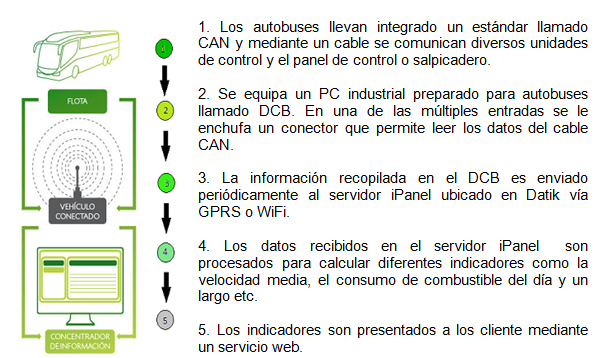
\includegraphics[width=1\textwidth]{Ilustraciones/ipanel_infraesctructure.png}
	\caption{Funcionamiento resumido de iPanel}
	\label{fig:ipanel}
\end{figure}

La incesante integración de nuevos vehículos a iPanel ha generado un crecimiento exponencial en el número de registros almacenados en ciertas tablas de MySQL. Aunque el volumen actual no suponga riesgo alguno para el funcionamiento del servicio, Datik tiene identificados varios escenarios en los que la situación se podría revertir, causando graves problemas en el sistema.\\

El primero de todos, es la corrupción de datos. Este fenómeno sucede debido a un bug, fallo de almacenamiento inesperado, o una caída de MySQL cuando el resultado del checksum de una página es diferente al esperado. Aunque ocurre de forma esporádica, compromete seriamente la información que Datik ofrece a sus clientes mediante la aplicación web.\\ 

Otro de los problemas, intrínseco a depender de una base de datos centralizada, es el operar sobre un único punto de fallo. Debido a que la mayoría de procesos confluyen en ella, el bloqueo o la caída causada por un servicio puede acarrear la de otros, a priori, totalmente independientes. Para solventar el problema Datik ha optado por migrar su infraestructura a una basada en Microservicios \cite{newman2015building}, logrando de esa manera, el aislamiento total de los componentes que conforman su ecosistema.\\ 

El último problema, es el referente al proceso denominado Cálculo de Indicadores, el cual se ejecuta una vez al día para realizar operaciones aritméticas sobre diversas tablas y después agrupa los resultados en base a diferentes criterios dependiendo del cliente. Siendo dichas tablas las que mayor crecimiento experimentan, el aumento del volumen de las mismas incrementa de forma desorbitada el tiempo necesario para finalizar el cálculo, pudiendo, en un futuro, llegar a tardar mas de 24 horas y cancelar los indicadores que ofrecen información del último día.\\

Siendo los indicadores parte vital de la información que se despliega vía iPanel, el presente proyecto ofrece una solución tecnológica para poder escalar horizontalmente la infraestructura solventando así el problema de almacenamiento y ...   

En las proximas lineas se (buscar solucion a los problemas mencionados, sobre todo el ultimo que se encuentra sin solucion visible)

\section{Propuesta}

*la escalabilidad vertical de la máquina no es la solucion viable a largo plazo
*algunos de esos problemas ya empiezan a ser palpables
* problema en el que nos centramos en este proyecto
* requiere de una respuesta tecnologica
* requiere de tecnologia que datik no cuenta

* Palabras de henry ford
* esfuerzo enorme en tunear mysql, no conviene

* Diseccionar el problema: almacenamiento y procesamiento

Para solventar los problemas que Datik prevé, se propone implantar las tecnologías Apache Cassandra y Apache Spark en la empresa y migrar tanto las tablas como los procesos que son parte en el cálculo de los indicadores.\\


Apache Cassandra es una base de datos distribuida no-sql. Gracias a naturaleza distribuida ayuda a resolver, 

Funcionalidades nuevas que trabajan con videos etc




Diseñar un plan de migración que defina aspectos tales como: 

\begin{itemize}
	\item Listado de las tablas MySQL que deben ser migradas a Cassandra priorizando las que más rápido crecen y mayor número de consultas intensivas reciben. Por ejemplo, las tablas que contienen la información para el calculo de los indicadores.
	\item Listado tablas "frontera"
	\item Ver por cada ejercicio su estado de realización: quiénes lo han terminado, quiénes tienen duda y quiénes no han respondido nada.
	\item Editar cualquier detalle de un ejercicio en cualquier momento.
	\item Valorar la realización de un ejercicio a un alumno concreto.
\end{itemize}

el traspaso de las tablas MySQL que mayor velocidad crecen  y mayor número de consultas pesadas reciban a estas nuevas tecnologías. empezando por las que tienen estrecha realción con el calculo de indicadores, ya que, como se ha indicado con anterioridad, es  

Por su parte, Apache Cassandra

Por Apache Spark por otra,

Debido a la falta de datos se ha utilizado un dataset publico para emular las condiciones de futuro con las que se va a encontrar datik

\section{Organización del documento}

En esta memoria se ha documentado  el desarrollo de la herramienta \textbf{\textit{exerClick}}, dentro del Trabajo de Fin de Grado (TFG) del autor. En el documento se describe la propuesta, la planificación y gestión que esta lleva consigo, la implementación llevada a cabo y las conclusiones finales.\\

En este primer capítulo se ha introducido el problema a resolver y se ha explicado la propuesta presentada en este proyecto.\\

En el capítulo 2 se presenta el Documento de Objetivos de Proyecto (DOP). Este recoge el alcance y las fases y tareas del proyecto, el análisis de riesgos y el análisis de factibilidad.\\

Una vez en el capítulo 3 se explica la gestión llevada a cabo durante el proyecto. Se presentan las metodologías utilizadas: Metodologías Ágiles e InterMod (adaptada a las necesidades de este proyecto). A continuación se detallan cada una de las iteraciones llevadas a cabo (como parte de la metodología InterMod): duración, objetivos y tareas realizadas. Al final del capítulo se muestra la documentación asociada a las iteraciones y los objetivos, además del seguimiento de tiempo realizado.\\

A continuación, en el capítulo 4 se detalla el análisis de requisitos. Primero se detallan los requisitos no-funcionales y luego los funcionales (prototipos en papel llevados a cabo durante las primeras iteraciones que dan una visión global del proyecto).\\

En el capítulo 5 se explica el diseño e implementación llevados a cabo. Se comienza mostrando la estructura de documentos del proyecto, luego el diseño realizado en base al análisis de requisitos del capítulo 4 y finalmente una visión general de la implementación de la lógica de negocio.\\

Para finalizar, en el capítulo 6 se presentan las conclusiones, líneas futuras para el proyecto y las lecciones aprendidas.\\

Fuera de la estructura general de la memoria, tenemos la bibliografia y los apéndices. En estos últimos tenemos las actas de reuniones, las actas de pruebas y la vista de relaciones de la base de datos (de la parte utilizada o creada específicamente para el proyecto).\\

%----------------------------------------------------%
%    FUNCIONAMIENTO DE LAS TÉCNOLOGIAS PROPUESTAS    %
%----------------------------------------------------%

\cleardoublepage
%----------------------------------------------------%
%       ANÁLISIS DE LAS TÉCNOLOGÍAS PROPUESTAS       %
%----------------------------------------------------%

\pagestyle{fancy}

\chapter{Análisis de las tecnologías propuestas}
\label{analisis_tecnologias}

\section{Apache Cassandra}

Apache Cassandra es una base de datos distribuida que permite operar sobre grandes volúmenes de datos del tipo clave/valor. Concebida en el 2008 por los ingenieros de Facebook basándose en otros sistemas de almacenamientos distribuidos como Dynamo (Amazon) \cite{decandia2007dynamo} y BigTable (Google) \cite{chang2008bigtable}, se caracteriza por ofrecer una  disponibilidad total y mayor escalabilidad lineal en comparación a otras bases de datos NoSQL.  Para ello, se basa en un conjunto de nodos homogéneos dentro de una red en anillo que se comunican mediante un protocolo P2P de replicación asíncrona, lo cual permite realizar operaciones de baja latencia para todos los clientes sin necesidad de un servidor maestro.\\

Hoy en día, es utilizada por infinidad de aplicaciones en negocios modernos, siendo la base de datos elegida por un tercio de las compañías que conforman la Fortune 100 \footnote{\url{http://fortune.com/2015/04/14/datastax-hp-sales-partnership/}}. Claro ejemplo de ello son empresas mundialmente conocidas como Apple, Facebook o NetFlix, los cuales utilizan Apache Cassandra como parte de su entramado tecnológico desde hace ya unos años. Cabe destacar que su uso no se limita al mundo empresarial. Muestra de ello es la acogida que ha tenido en el ámbito de la investigación, formando parte en experimentos punteros a nivel mundial como algunos de los realizados en el CERN \cite{sicoe2012persistent}.\\

\subsection{Funcionamiento}

Las bases de datos NoSQL, en su mayoría, han sido concebidas para lidiar con un conjunto especifico de problemas. Debido a ello, para entender el funcionamiento de Apache Cassandra se ha decidido resaltar las peculiaridades que le distinguen de los demás sistemas de almacenamiento no relacionales.

\subsubsection{Base de datos distribuida de alta disponibilidad}

El Teorema de Brewer \cite{gilbert2002brewer}, también conocido como Teorema CAP , enuncia que un sistema de cómputo distribuido no puede  garantizar simultáneamente las tres propiedades que se presentan a continuación, solo pudiendo cumplir dos de ellas al mismo tiempo, y acabar cumpliendo la restante tarde o temprano:

\begin{itemize}
	\item \textbf{Consistencia}(Consistency): Todos los nodos ven la misma información al mismo tiempo.
	\item \textbf{Disponibilidad}(Availability): La garantía de que cada petición a un nodo reciba una confirmación de si ha sido o no resuelta satisfactoriamente.
	\item \textbf{Tolerancia al Particionado}(Partition Tolerance): El sistema sigue funcionando a pesar de que haya sido partido por un fallo de red.
\end{itemize}

Para una base de datos distribuida que promete la disponibilidad completa, el Teorema de Brewer implica la incapacidad de garantizar la consistencia total de los datos que almacena y la necesidad de esperar un tiempo indeterminado para que las réplicas de un registro modificado se actualicen correctamente.\\

Para lidiar con dicha restricción, Cassandra ofrece la posibilidad de afinar el nivel de consistencia \footnote{\url{https://docs.datastax.com/en/cassandra/2.1/cassandra/dml/dml_config_consistency_c.html}} en cada consulta sacrificando para ello parte de la disponibilidad. Así, las consultas de mayor disponibilidad responden con el dato ofrecido por la primera réplica sin siquiera cotejar la existencia de una versión actualizada del mismo, mientras que las consultas de mayor consistencia pueden corren el riesgo de fallar si algún nodo caído provoca que no se pueda satisfacer el nivel de consistencia requerido. Por tanto, queda en manos del diseñador el trabajo de encontrar el equilibrio entre ambas características, siendo la naturaleza de los datos a tratar un factor determinante para ello.

\subsubsection{Optimizado para escrituras}

Una de las características a destacar de Cassandra es el elevado ratio de escrituras por segundo que es capaz de realizar, superando notoriamente a otras bases de datos NoSQL en este apartado \cite{rabl2012solving}.

Al ejecutar una consulta que desemboca en una escritura, los registros son almacenados en dos estructuras denominadas CommitLog y Memtable. El primero, es un fichero donde se adjuntan los registros recibidos, mientras que el segundo, es una cache en memoria que apila dichos registros hasta llegar a su capacidad máxima. Cuando ambas estructuras finalizan de almacenar los datos, Cassandra considera que la consulta ha sido ejecutado satisfactoriamente pudiendo pasar a procesar otras operaciones.\\

Cuando la Memtable se llena empieza un proceso de vaciado en el cual, primero, se dilucida el nodo destinatario de cada registro. Después, dichos registros son escritos de forma secuencial en estructuras inmutables denominadas SSTable, ficheros que representan físicamente el contenido de una tabla en Cassandra. Si esta operación es interrumpida, se utiliza la información almacenada en el CommitLog para recuperar las escrituras perdidas. Finalmente, cuando todos los registros han sido transferidos a su correspondiente SSTable, el CommitLog es purgado.\\

\begin{figure}[h]
	\centering
	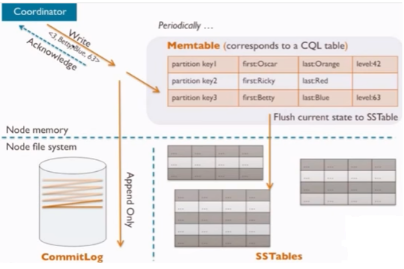
\includegraphics[width=0.65\textwidth]{Ilustraciones/cassandra_data_storage.png}
	\caption{Almacenamiento de datos en Cassandra}
	\label{fig:almacenamiento_cassandra}
\end{figure}

Debido a la naturaleza inmutable de las SSTable, cada vez que la Memtable se vacía un nuevo fichero es generado para representar una misma tabla. Ello puede acarrear problemas de eficiencia a la hora de consultar la información de dicha tabla, ya que será totalmente necesario leer todos los ficheros correspondientes. Para sobreponerse a este inconveniente, Cassandra posee un mecanismo llamado compactación que unifica las SSTable que representan una misma tabla eliminando los ficheros restantes.\\

\subsubsection{Replicación asíncrona sin maestro}

Las bases de datos distribuidas ofrecen la posibilidad de replicar los datos que se almacenan en ella, asegurando una respuesta satisfactoria a las peticiones aún habiendo nodos inactivos en la infraestructura. Ello implica la necesidad de conocer el estado de las réplicas y otras maquinas por parte de cada nodo del sistema, que por lo general, se resuelve mediante un modelo maestro-esclavo.\\

En Cassandra, gracias a un conjunto de mecanismos peer-to-peer, cada nodo es capaz de obtener dicha información de forma local sin depender de un nodo maestro, obteniendo un clúster totalmente homogéneo.\\ 

\textbf{Gossip Protocol}\cite{demers1987epidemic}: Protocolo de comunicación peer-to-peer que intercambia el estado del propio nodo y de aquellos que conoce de forma periódica.\\

Cada mensaje Gossip tiene una versión asociada a él, gracias al cual el nodo que recibe dicho mensaje puede comparar con la información que tiene de antemano y actualizar su conocimiento en caso de ser necesario.\\

 En el caso concreto de Cassandra, el intercambio se realiza cada segundo entre los nodos vecinos, logrando así que, al propagarse la información por el anillo, todos los nodos del clúster aprendan sobre el resto de manera rápida.\\

\textbf{Failure Detector}\cite{chandra1996unreliable}: Conjunto de métodos que usando mensajes Gossip sugieren de forma local si otro nodo del sistema esta caído o en estado transitorio.\\

Entre todos los métodos existentes, Cassandra utiliza el Accrual Failure Detector\cite{hayashibara2004spl}. Además ofrece la posibilidad de configurar un umbral por cada nodo que tenga en cuenta el rendimiento de red, carga de trabajo, u otras condiciones. Al cotejar el valor ofrecido por el detector con dicho umbral, Cassandra es capaz de dilucidar si un nodo esta caído, y en caso afirmativo, redireccionar las peticiones a otro activo.\\

// merkle tree (paper?)

Consiste en comparar todas las réplicas de cada dato que existe o debería existir y actualizarlos a la versión más reciente mediante el uso de Merkle Trees.

Un Merkle tree es un árbol de hash donde los nodos padres más altos en el árbol son los hashes de sus respectivos hijos. La ventaja principal de árbol de Merkle es que cada rama del árbol se puede comprobar de forma independiente , sin la necesidad de descargar todo el conjunto de datos.

La implementación de Anti-Entropia de Cassandra genera un Merkle tree por cada column family a la hora de la compactación y se almacenan solo hasta enviarlos a los nodos vecinos. 

Implica enviar un exceso de datos por la red pero ahorra en operaciones I/O del disco local, lo cual es preferible para conjuntos de datos muy grandes.

\subsubsection{Sin punto único de fallo}

//replicacion factor + diapositivas

///

A la hora de definir un keyspace dos atributos estrechamente relacionados han de ser especificados: Replication Factor y Replica Placement Strategy(). El primero, consiste en un número que indica cuantas copias de un mismo registro se han de almacenar en la infraestructura. Cada nodo posee una réplica para un cierto rango de datos y si uno de ellos falla, otro que posea dicha réplica puede responder a la petición sin tener que interrumpir el servicio. El segundo, define cómo se han de repartir los registros replicados por el anillo, ofreciendo distintas opciones dependiendo si los nodos del clúster se encuentran alojados en un único datacenter o repartidos entre varios.\\

El atributo Replica Placement Strategy cobra especial interés al operar sobre un clúster cuyos nodos están distribuidos en punto geográficos lejanos, ya que permite almacenar cada réplica en diferentes puntos del globo. De esa manera, se consigue minimizar la latencia de las peticiones recibidas desde diferentes puntos del plantea y además, proteger la base de datos de una posible caída a nivel de datacenter debido a diversos catástrofes.\\ 

Si un componente de Cassandra tiene especial importancia en su funcionamiento es el ColumFamily. En una base de datos relacional como MySQL, las tablas son diseñadas con el objetivo de minimizar la redundancia de los datos almacenados en ella, siguiendo para lograr dicho objetivo un proceso de normalización[]. En cambio, al operar con Cassandra, ocurre exactamente lo contrario. Las tablas se construyen buscando una respuesta rápida a las consultas sin importar que ello implique tener que almacenar datos redundante en la base de datos.\\

patition key etc



\begin{figure}[h]
	\centering
	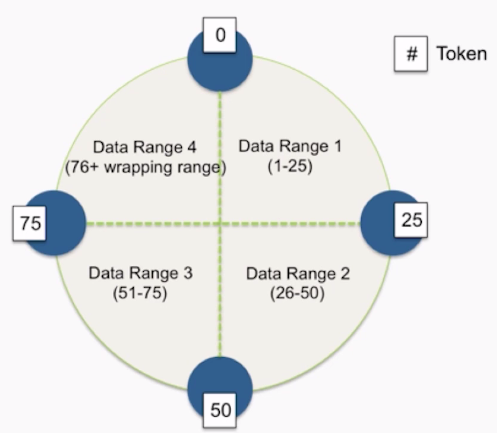
\includegraphics[width=0.5\textwidth]{Ilustraciones/cassandra_token.png}
	\caption{Particionamiento en Cassandra}
	\label{fig:cassandra_token}
\end{figure}

consecuencia: restriccion en las consultas que se pueden realizar

\subsection{Cassandra Query Lenguage (CQL)}

permite conectarse al cualquier nodo del cluter (homogeneidad)

Apache Cassandra posee su propio lenguaje de consultas, el denominado Cassandra Query Lenguage (CQL). Su sintaxis guarda una gran similitud con la de SQL, lo cual facilita, de forma notoria, el salto que supone pasar de trabajar con bases de datos relacionales a distribuidos.\\

Aún siendo sintácticamente  tan parecido a SQL, presenta ciertas restricciones debido a que es un lenguaje de consultas de una base de datos distribuida. Por ejemplo, no ofrece la posibilidad de realizar operaciones como JOIN y es totalmente necesario especificar todas los atributos que componen la clave primaria a la hora de realizar cualquier consulta de filtrado o de actualización en la tabla. La única operación que no cumple esta restricción es un select que contenga la clausula where, ya que, al definir la clave primaria Cassandra indexa de forma automática todos sus componente, posibilitando más tarde  hacer uso de ellos en este caso concreto.

Otra de las peculiaridades que presenta CQL es el hecho de ofrecer dos modos distintos de realizar un update. El primero de todos es el mencionado en el párrafo anterior. El segundo posibilita actualizar una columna realizando un insert repitiendo el valor de las claves primarias de una columna ya existente en la base de datos. Esta segunda forma es cómoda a la par de peligrosa porque Cassandra no notifica si una clave primaria ya existe en la base de datos o no, pudiendo un insert desencadenar en un update no deseado.  

\section{Apache Spark}

Apache Spark[9] es un proyecto open source de computación en clúster. Desde el principio fue diseñado para poder ejecutar algoritmos iterativos en memoria sin la necesidad de almacenar en disco los resultados intermedios generados durante el proceso. Esta peculiaridad permite que los procesamientos llevados a cabo con Spark puedan llegar a ser, en algunos casos concretos, 100 veces más rápidos que los de MapReduce[10].\\

A mediados de 2014, coincidiendo con el lanzamiento de la primera versión, alcanzó la cifra de 465 colaboradores, convirtiéndolo en el proyecto más activo entre los relacionados con el Big Data dentro de la Apache Software Fundation.\\

Apache Spark está compuesto por múltiples y variados componentes que pueden ser utilizados de forma conjunta.\\

\begin{figure}[h]
	\centering
	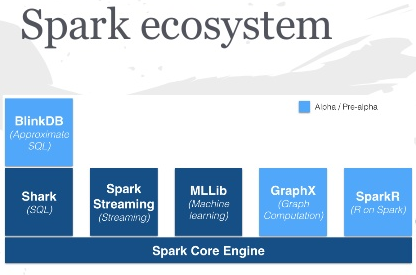
\includegraphics[width=0.5\textwidth]{Ilustraciones/spark_ecosystem.png}
	\caption{Ecosistema Spark}
	\label{fig:ipanel}
\end{figure}

La base del proyecto es el denominado Spark Core. Proporciona envío distribuido de tareas, planificación y funciones básicas de entrada salida. La abstracción fundamental de programación se llama Resilient Distributed Datasets (RDD)[11], una colección lógica de datos particionados a través de las máquinas que se expone mediante una API integrada en lenguajes como Java, Python y Scala.\\

\subsection{Funcionamiento}

Para el funcionamiento de Spark, es condición sine qua non que los nodos de la infraestructura tengan acceso a la totalidad de los datos que se desea tratar. Ello implica que para procesar un fichero de 50GB, cada nodo tendría que poseer una copia del mismo almacenado en su disco. Esta praxis es inviable, ya que más allá de los problemas de consistencia que generaría, para nada es eficiente ocupar la memoria de todos los nodos con información redundante y procesar el fichero entero cuando en realidad se va a hacer uso de una pequeña porción de dichos datos en cada ejecución.\\

Las bases de datos distribuidas como Cassandra solventan los problemas anteriormente mencionados. Se encargan de distribuir los datos entre diferentes nodos del clúster, ofrecen la posibilidad de acceder a ellos desde cualquier punto y mantienen la consistencia de los mismos a cambio de sufrir una pequeña latencia en el caso de requerir información almacenada en otro nodo de la infraestructura.\\ 

Al ejecutar una aplicación que opera con Spark, un componente denominado driver es lanzado. Debido a la necesidad de obtener recursos (CPU y memoria) para llevar a cabo la computación que se le ha encomendado, se comunica con un nodo del clúster que, mediante especificación previa, adopta el rol de maestro. Éste pregunta a todos los nodos que conforman la infraestructura sobre la cantidad de recursos disponibles que poseen y así asignarles los executors correspondiente. Las máquinas que alojen al menos un executor pasan a denominarse worker y a partir de este momento, cada executor podrá comunicarse directamente con el Driver para poder recibir las tareas que éste le envíe.\\

Un executor es una unidad de trabajo que se encarga de computar las tareas que le encomienda el driver. El número de executors que puede albergar cada worker está directamente relacionado con el número de procesadores que este posee. De la misma forma, es posible repartir la memoria RAM que dispone el nodo worker entre varios executors. Spark permite modificar ambos parámetros programáticamente permitiendo así poder amoldarse a las particularidades de cada ejecución.\\

Para transferir el código del programa, residente en la máquina del driver, éste adopta  el rol de servidor e intenta enviar dicho código a los workers. Si el fichero JAR que contiene el código ha sido recibido correctamente por sus destinatarios, estos responden mediante un ACK y en caso contrario, se vuelve a intentar el envío un número determinado de veces. Una vez llegado al máximo de reintentos, el worker que no haya enviado el ACK es considerado como caído, quedando los executors que albergaba fuera del posterior reparto de tareas.\\

\begin{figure}[h]
	\centering
	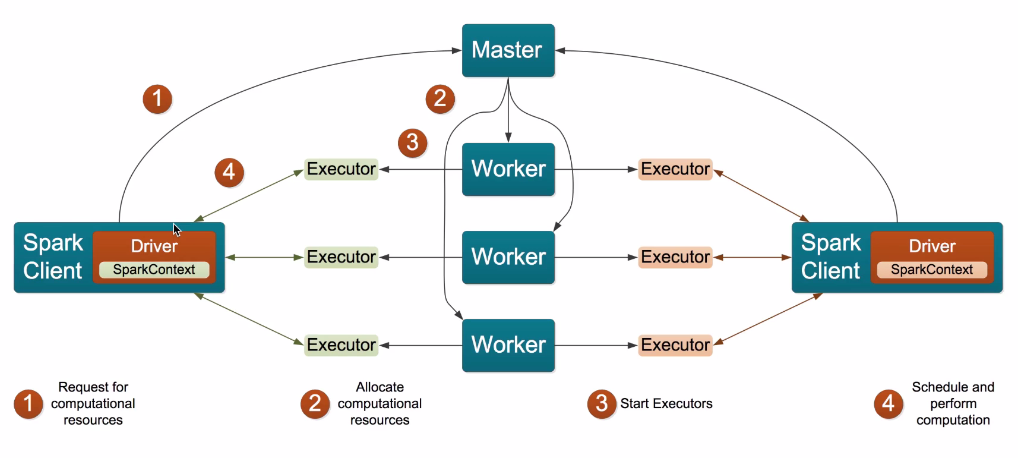
\includegraphics[width=1\textwidth]{Ilustraciones/spark_architecture.png}
	\caption{Arquitectura Spark}
	\label{fig:spark_architecture}
\end{figure}

A la hora de realizar operaciones en Spark, el objeto estrella es el denominado Resilient Distributed Datasets (RDD)[11]. Se trata de una abstracción que mediante diferentes APIs disponibles para Java, Scala y Python permite manipular datos distribuidos por los diferentes nodos del clúster como si estuvieran almacenados de forma local. Este objeto es inmutable, lo cual implica que una vez creado no se le pueden añadir nuevos elementos o eliminar los existentes, solo aplicar transformaciones y acciones sobre el.\\

Las operaciones que se pueden realizar sobre las RDD se agrupan, tal y como se ha adelantado antes, por transformaciones y acciones. Las primeras transforman un RDD en otro según el criterio indicado y las segundas realizan modificaciones sobre los datos almacenados en dichas RDD. Cabe destacar que las transformaciones en Spark son operaciones "lazy", lo cual implica que en realidad cada nodo memoriza la secuencia de transformaciones que ha de realizar y los procesa cuando una acción es ejecutada.\\

Una vez terminada la primera fase en la que los executor son creados y enlazados con el driver, éste último empieza a analizar la estructura del código y genera un grafo DAG (Directed Acyclic Graph) con las operaciones que se realizan sobre la RDD. Partiendo de ese grafo genera un job por cada operación de tipo acción que encuentra y dentro de cada job separa la ejecución en diferentes stages según las dependencias que existan entre operaciones. Por último, cada stage es dividido por defecto en unidades de 64MB y a cada unidad resultante se denomina task, el cual es enviado a un executor para ser procesado. El tamaño de cada task puede ser modificado programáticamente, pudiendo de esa forma manipular el número de task que un executor deba ejecutar.\\

\begin{figure}[h]
	\centering
	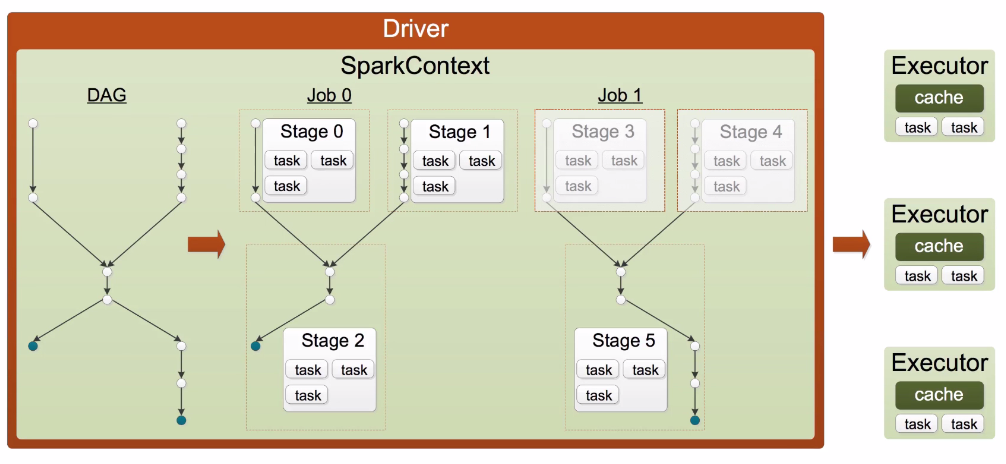
\includegraphics[width=1\textwidth]{Ilustraciones/spark_task_creation.png}
	\caption{Arquitectura Spark}
	\label{fig:spark_task_creation}
\end{figure}

El driver, una vez habiendo recibido los resultados de todas los task que ha repartido, enviará un mensaje a los executors indicando que el procesamiento ha sido finalizado y calculará el resultado final ofreciendo la posibilidad de, por ejemplo, almacenarlo en una base de datos distribuida como Cassandra.\\








%----------------------------------------------------%
%         ENTORNO DE PRUEBAS: CONSTRUCCION           %
%----------------------------------------------------%

\cleardoublepage
%%----------------------------------------------------%
%          ENTORNO DE PRUEBAS: CONSTRUCCION          %
%----------------------------------------------------%

\pagestyle{fancy}

\chapter{Entorno de pruebas: Construcción}
\label{entorno_pruebas}

Conocedores de la problemática a solventar y de las tecnologías que se desean utilizar para ello, es momento de detallar la confección de los entornos de prueba utilizados para medir el rendimiento de dichas tecnologías.\\

En las siguientes páginas, se describe, por un lado, la construcción de un entorno centralizado compuesto por un único nodo que alberga instancia de MySQL Server, cuyo objetivo es imitar la infraestructura monolítica que impera en Datik. Por el otro lado, se expone el ensamblaje de un entorno distribuido, formado por tres nodos homogéneos sobre los cuales operan Apache Cassandra y Apache Spark en consonancia.\\

Dichos nodos son erigidos mediante máquinas virtuales que operan sobre distintos dispositivos. Los procesos clientes se alojan en un ordenador portátil mientras que las instancias relativas a los servidores se ejecutan sobre un ordenador de sobremesa, logrando así neutralizar toda diferencia que pudiese existir en cuanto a hardware. Para dar comienzo a este tercer capítulo, se describen las características físicas de los dispositivos recién mencionados.

\clearpage

\section{Características de las máquinas físicas}

\textbf{Ordenador portátil}: Terminal que alberga los procesos cliente encargados de lanzar diversas peticiones contra el servidor y recolectar los resultados computados por este, además de cuantificar el tiempo transcurrido entre ambos eventos.

\begin{itemize}
	\item Procesador: Intel(R) Core(TM) i-5 4200M CPU @ 2.50 GHz
	\item Memoria RAM: 8 GB
	\item Disco Duro: Western Digital WD5000LPCX-24C6HTO SSD 500GB
	\item Sistema Operativo: Windows 10
	\item Adaptador Red: Qualcomm Atheros AR8172/8176/8178 PCI-E Fast Ethernet Controller (NDIS 6.30)
\end{itemize}

\textbf{Ordenador de sobremesa}: Terminal que adquiere el rol de servidor dentro del entramado. Se encarga del almacenamiento y procesamiento de los datos mediante el uso de las tecnología que se analizan en el presente proyecto.

\begin{itemize}
	\item Procesador: AMD FX(tm)-8350 Eight-Core Processor 4.00GHz
	\item Memoria RAM: 32 GB
	\item Disco Duro: Western Digital WD5000AAKX-22ERMA0 SSD 500GB
	\item Sistema Operativo: Windows 10
	\item Adaptador Red: Killer e2200 Gigabit Ethernet Controller (NDIS 6.30)
\end{itemize}

Ambas máquinas se encuentran enlazadas a un \textit{switch} tp-link-tl-sf1008d mediante sendos conectores Fast Ethernet, permitiendo intercambiar datos a una velocidad de 100 Mb/s.\\

El switch, a su vez, está conectado a un \textit{router} que proporciona acceso al exterior de la red privada, el cual sólo será utilizado para descargar contenido relativo a los preparativos de las pruebas.

\clearpage

\section{Confección de las máquinas virtuales}
 
Con el objetivo de no realizar las mismas configuraciones reiteradamente, se ha decidido crear una máquina virtual básica siguiendo los pasos que se describen a continuación y tras su puesta a punto, clonarla tantas veces como instancias hagan falta.

\begin{enumerate}
	
	\item \textbf{Crear la máquina virtual}: Instancia creada mediante VirtualBox utilizando la imagen de Ubuntu Server 16.04 LTS y 75 GB de memoria física. El resto de las características no han sido especificadas ya que es posible reasignar su valor en cualquier momento.
	
	\item \textbf{Asignar una IP estática}: La mayoría de los clones generados sobre esta máquina adquieren el rol de servidor, por lo que no es de recibo que su IP pueda variar cada vez que el servicio de red o la máquina misma se reinicien. Para evitar cualquier inconveniente de este estilo, es totalmente necesario configurar una interfaz de red con una IP estática.
	
	\item \textbf{Cambiar el adaptador de red a modo puente}: Al crear una máquina virtual con VirtualBox, el adaptador de red predefinido es el NAT. Ello implica que dicha máquina se encontrará aislada en una red lógica y solo podrá acceder a otros dispositivos pasando por la máquina física y haciendo uso de su IP.\\
	
	Modificando el adaptador de red al modo puente se consigue extender la red privada hasta el nodo virtual, eliminando así toda dependencia con la máquina física y posibilitando la comunicación con el resto de los dispositivos que residen en la misma red privada.
	
	\item \textbf{Instalar Java 8}: Las tecnologías que se desean probar en las futuras pruebas se ejecutan sobre la Máquina Virtual de Java(JVM), por lo que es necesario instalar una versión de Java para su funcionamiento. Entre todas las disponibles se ha optado por la versión 8.
	
\end{enumerate}

Una vez terminado de confeccionar la máquina virtual básica, es aconsejable ejecutar el comando \textit{tracert} y comprobar ciertas métricas como la latencia y el número de saltos que se dan por la red hasta llegar a otro nodo de la infraestructura. Siguiendo este simple consejo es posible identificar errores relacionados con la configuración y solucionarlos con mayor celeridad.

\clearpage

\section{Entorno centralizado}

El objetivo del entorno centralizado es imitar la infraestructura utilizada por Datik para ejecutar el proceso Cálculo de Indicadores. Dicha infraestructura consta de un servidor en la nube que alberga una instancia de MySQL Server y un proceso que actúa como cliente. Este último realiza consultas contra la base de datos y computa los registros obtenidos para calcular los indicadores deseados.

\subsection{Servidor}

La creación y confección del nodo servidor para el entorno de pruebas centralizado se resume en los siguientes pasos:

\begin{enumerate}
	
\item \textbf{Clonar la máquina virtual base}: Crear una copia de la instancia básica confeccionada en el apartado anterior y asignar los parámetros especificados en cuadro \ref{nodo-mysql} de la página \pageref{nodo-mysql}.

\begin{table}[h!]
	\centering
	\begin{tabular}{|l||l|l|l|}
		
		\hline
		
		& \textbf{IP Privada} & \textbf{Procesadores} & \textbf{Memoria RAM} \\
		
		\hline
		\hline
		
		Nodo MySQL & 192.168.0.100 & 6 & 24 GB \\
		
		\hline
		
	\end{tabular}
	\caption{Descripción del nodo centralizado}
	\label{nodo-mysql}
\end{table}

\item \textbf{Descargar e instalar la última versión de MySQL}: Acceder a la máquina virtual recientemente clonada e instalar la última versión de MySQL Server, la 5.7, mediante Advanced Packaging Tool (APT) de Ubuntu.

\item \textbf{Crear un esquema}: Identificarse contra MySQL Server utilizando el único usuario existente por el momento, 'root', y la contraseña que se le ha asignado durante la instalación para crear el esquema encargado de almacenar los datos.

\item \textbf{Posibilitar acceso desde la máquina remota}:  Por motivos de seguridad, las aplicaciones que se conectan a la base de datos no deberían de acceder a ella mediante el usuario 'root', por lo que se recomienda crear un nuevo usuario y especificar los permisos que este ha de tener sobre el esquema creado en el paso anterior.

\item \textbf{Abrir los puertos necesarios}: Al estar trabajando sobre máquinas virtuales alojadas en una red propia, todos los puertos se encuentran abiertos por defecto, pero en caso de existir algún cortafuegos que protegiera el servidor, sería necesario abrir el acceso al puerto donde escucha MySQL, el 3306 por defecto.

\end{enumerate}

\subsection{Emulando el cliente}

Emular un proceso cliente en el entorno centralizado es tan simple como instalar la última versión del MySQL Workbench\footnote{\url{https://www.mysql.com/products/workbench/}} sobre el ordenador portátil (no hace falta máquina virtual alguna) y crear una nueva conexión con el servidor especificando la IP junto al usuario y contraseña correspondientes.

\section{Entorno distribuido}

Infraestructura cuyo núcleo es un clúster compuesto por tres nodos virtuales alojados en el ordenar de sobremesa erigido con el objetivo de almacenar y procesar el dataset de prueba.\\ 

Un proceso cliente residente en el ordenar portátil, por su parte, se encarga de ejecutar el programa que especifica el procesamiento que ha de llevar a cabo el clúster y cuantificar el tiempo transcurrido en dicha tarea.

\subsection{Servidor distribuido}

En las siguientes líneas se detalla la configuración de los nodos que conforman el clúster y la puesta a punto de las tecnologías que operan sobre él.

\begin{enumerate}
	
\item \textbf{Clonar la máquina virtual base}: Clonar la máquina virtual base tantas veces como nodos vayan a conformar la infraestructura. En éste particular caso se crean 3 copias.\\

Además de configurar la IP, el número de procesadores y la memoria RAM disponible para cada uno, es necesario hacer lo propio con el hostname. Apache Cassandra recurre a este atributo para conocer la IP de una máquina cuando ciertos elementos del fichero de configuración no son especificados y en el caso de Spark, el proceso \textit{driver} utiliza los hostname para establecer la conexión con otros nodos de la infraestructura. El cuadro \ref{nodos-cluster} de la página \pageref{nodos-cluster} resume la asignación de dichos atributos.\\

\begin{table}[h!]
	\centering
	\begin{tabular}{|l||l|l|l|l|}
		
		\hline
		
		& \textbf{IP Privada} & \textbf{Procesadores} & \textbf{Memoria RAM} & \textbf{Hostname} \\
		
		\hline
		\hline
		
		Nodo 1 & 192.168.0.101 & 2 & 8 GB & nodo1 \\
		
		\hline
		
		Nodo 2 & 192.168.0.102 & 2 & 8 GB & nodo2 \\
		
		\hline
		
		Nodo 3 & 192.168.0.103 & 2 & 8 GB & nodo3 \\
		
		\hline
		
	\end{tabular}
	\caption{Descripción de los nodos que componen el clúster}
	\label{nodos-cluster}
\end{table}

Cabe destacar que la suma de recursos físicos destinados a la creación del clúster es idéntica a los recursos destinados para erigir el servidor del entorno centralizado.

\item \textbf{Resolver hostnames a IPs}: Los hostname recién configurados no sirven de nada si no es posible asociarlos a una IP concreta. Dicho trabajo lo suele realizar un DNS, pero al estar operando sobre una red privada que no dispone de DNS alguno, es necesario recurrir al fichero \textit{/etc/hosts} para obtener la información deseada. Este fichero debe de albergar la IP privada y el hostname de la propia máquina y del resto de hosts que conforman el clúster.

\item \textbf{Descargar Apache Cassandra}: Puede ser instalada mediante paquetes deb o rpm pero en este proyecto se ha optado por descargar el archivo binario y ejecutarlo de forma manual una vez realizadas las configuraciones pertinentes.\\ 

Siendo un proyecto de código abierto relativamente reciente, las nuevas versiones y actualizaciones son lanzadas frecuentemente para arreglar bugs e implementar funcionalidades nuevas. Debido a ello, es imposible trabajar con la última versión, por lo que se ha decidido utilizar la 2.1.8 para el desarrollo del presente proyecto.

\item \textbf{Descargar Apache Spark}: Es necesario tener en cuenta la compatibilidad con la versión de Cassandra ya descargada. Aunque en principio se trata de dos proyectos totalmente independientes, existen conectores que buscan facilitar un uso conjunto de estas tecnologías. Analizando la tabla de compatibilidades\footnote{\url{https://github.com/datastax/spark-cassandra-connector}} ofrecida por DataStax, dueña del conector seleccionado para el presente proyecto, se ha decidido descargar la versión 1.4.1 de Spark.
	
\end{enumerate}

\subsubsection{Configuración de Apache Cassandra}

El fichero que alberga todos los atributos configurables de Cassandra es el denominado  \textit{cassandra.yaml} y se encuentra alojado dentro de la carpeta \textit{conf}. Es necesario modificar en cada uno de los nodos que conforman el clúster, los atributos que se definen a continuación:

\begin{itemize}

\item \textbf{cluster\_name}: Varios clúster lógicos pueden coexistir dentro de uno físico. Éste atributo permite determinar a cual de todos pertenece el nodo.

\item \textbf{initial\_token y num\_token}: Al insertar un registro, un proceso denominado \textit{partitioner}\footnote{\url{https://docs.datastax.com/en/cassandra/2.1/cassandra/architecture/architecturePartitionerAbout_c.html}} se encarga de dilucidar en cual de los nodos se ha de almacenar. Para ello, cada nodo tiene que conocer de antemano el rango de particiones que se le han atribuido, especificado mediante el atributo initial\_token.\\

No obstante, remover o añadir nuevos nodos en el sistema implica volver a calcular y modificar dicho rango en cada máquina; tarea inviable cuando la envergadura del clúster aumenta considerablemente. Para automatizar las operaciones mencionadas, las versiones más reciente de Cassandra añaden el concepto de nodos virtuales\footnote{\url{http://docs.datastax.com/en/cassandra/2.1/cassandra/architecture/architectureDataDistributeVnodesUsing_c.html}} y la opción de activar dicha funcionalidad mediante el atributo num\_token.

\item \textbf{seed\_provider}: Lista de direcciones IP delimitadas por coma que se utilizan como punto de contacto cuando un nodo desea unirse al clúster.

\item \textbf{listen\_address}: La dirección IP que utilizan otros nodos para conectarse a una máquina especifica. Si no se indica nada, el nombre de la máquina tiene que conducir a su IP utilizando el fichero \textit{etc/hostname}.

\item \textbf{rpc\_address}: La dirección IP de escucha para conexiones de cliente. Sus valores posibles son:

\begin{itemize}
	\item 0.0.0.0: Escucha en todas la interfaces configuradas
	\item Dirección IP
	\item Nombre de máquina
	\item Sin especificar: el nombre de la máquina tiene que conducir a su IP utilizando el fichero \textit{etc/hostname}
\end{itemize}

\item \textbf{endpoint\_snitch}: Establece el modo en el que Cassandra localiza nodos y envía peticiones de enrutamiento. Todos los nodos han de tener el mismo valor, siendo los siguiente los más utilizados:

\begin{itemize}
	\item SimpleSnitch: Se utiliza solo para la implementación de centro de datos únicos.
	\item RackInferredSnitch: Determina la ubicación de los nodos por rack o por data center.
\end{itemize}
	 
\end{itemize}
	 
\begin{table}[h!]
	\centering
	\begin{tabular}{|l||l|l|l|}
		
		\hline
		
		\textbf{Atributo} & \textbf{Nodo} 1 & \textbf{Nodo 2} & \textbf{Nodo 3} \\
		
		\hline
		\hline
		
		cluster\_name & Test Cluster & Test Cluster & Test Cluster \\
		
		\hline
		
		num\_token & 256 & 256 & 256 \\
		
		\hline
		
		seed\_provider & 192.168.0.102 & 192.168.0.101 & 192.168.0.101 \\ 
		               & 192.168.0.103 & 192.168.0.103 & 192.168.0.102 \\ 
		
		\hline
		
		listen\_address & 192.168.0.101 & 192.168.0.102 & 192.168.0.103 \\
		
		\hline
		
		rpc\_address & 192.168.0.101 & 192.168.0.102 & 192.168.0.103 \\
		
		\hline
		
		endpoint\_snitch & SimpleSnitch & SimpleSnitch & SimpleSnitch \\
		
		\hline
		
	\end{tabular}
	\caption{Configuración de los nodos Cassandra}
	\label{configuracion-nodos-cassandra}
\end{table}

Una vez habiendo configurado cada nodo de la forma indica en el cuadro \ref{configuracion-nodos-cassandra} de la página \pageref{configuracion-nodos-cassandra}, es necesario abrir los puertos detallados en el cuadro \ref{puertos-cassandra} de la página \pageref{puertos-cassandra} para que los procesos Cassandra puedan comunicarse entre los diferentes nodos que conforman el clúster.\\

\begin{table}[h!]
	\centering
	\begin{tabular}{|l||l|l|l|}
		
		\hline
		
		\textbf{Puerto} & \textbf{Descripción} \\
		
		\hline
		\hline
		
		7000 & Comunicación entre nodos utilizado en caso de no tener activado TLS \\
		
		\hline
		
		7001 & Comunicacion TLS entre nodos \\
		
		\hline
		
		7199 & Puerto para acceder a JMX \\ 
		
		\hline
		
		9042 & Puerto nativo de transporte para CQL \\
		
		\hline
		
		9160 & Cliente del API Thrift \\
		
		\hline
		
	\end{tabular}
	\caption{Puertos utilizados por Cassandra}
	\label{puertos-cassandra}
\end{table}

Para finalizar, es necesario arrancar los nodos uno a uno mediante el script \textit{cassandra.sh} que Cassandra mismo facilita dentro de la carpeta \textit{/bin} y comprobar que el clúster funciona correctamente utilizando la herramienta \textit{nodetool}\footnote{\url{http://docs.datastax.com/en/archived/cassandra/2.0/cassandra/tools/toolsNodetool_r.html}}.

\subsubsection{Configuración de Apache Spark}

Spark utiliza la memoria RAM de forma intensiva, por lo que se recomienda encarecidamente instalarlo en un clúster totalmente aislado al de Cassandra. No obstante, debido a que los recursos disponibles para lleva adelante el presente proyecto son limitados, no se ha podido seguir la recomendación y Spark ha sido instalado de tal forma que ambas tecnologías comparten nodo.\\

Al tratarse de un entorno de pruebas donde la cantidad de datos a manipular se encuentra predefinida, la instalación realizada no supone problema alguno y además ofrece diversas ventajas como el no tener que volver a configurar nuevas máquinas dentro del entramado, pudiendo pasar directamente a especificar las configuraciones relativas a Spark:

\clearpage

\begin{enumerate}
	
\item \textbf{Definir nodos esclavos}: El nodo maestro de Spark necesita saber qué máquinas están dispuestas a ofrecer sus recursos para un futuro procesamiento y poder alojar en ellas los \textit{worker} pertinentes. Para ello es necesario especificar las IP de dichos nodos en el fichero \textit{/conf/slaves}. Se ha de crear el directorio en caso de que no exista.

\item \textbf{Acceso entre máquinas mediante las claves RSA}: Spark sigue una arquitectura maestro/esclavo donde el maestro necesita conectarse a los esclavos para comunicar las operaciones que estos han de ejecutar. Para automatizar el proceso y evitar tener que introducir la contraseña cada vez que se quiera ejecutar algo, es necesario garantizar el acceso entre máquinas mediante las claves RSA.\\

Se recomienda crear los certificados con el comando \textit{ssh-keygen} y distribuirlos a los nodos cuya IP haya sido especificada en el fichero \textit{/conf/slaves} mediante el comando \textit{ssh-copy-id {usuario}@{servidor}} especificando el usuario que va a ejecutar el proceso Spark.

\item \textbf{Resolver hostnames a IPs}: Al instalar Cassandra se ha realizado el presente paso por lo que no hace falta volver a repetirlo. Aún así, cabe recordar que en caso de instalar Spark en un clúster independiente sería necesario manipular el fichero \textit{/etc/hosts} para especificar la IP privada y el hostname de la propia máquina y del resto de hosts que conforman el clúster.

\item \textbf{Definir el nodo Maestro}: Los nodos esclavos necesitan conocer la IP del terminal que adquiere el rol de maestro para poder aceptar las tareas enviadas por este último. Ello se consigue modificando  el fichero \textit{conf/spark-env.sh} y añadiendo las líneas \textit{SPARK\_MASTER\_HOST=ip\_del\_host} y \textit{SPARK\_LOCAL\_IP=ip\_del\_host} en cada una de ellas.
	
\end{enumerate}

Antes de iniciar el proceso es necesario cerciorarse de que los puertos mostrados en el cuadro \ref{puertos-spark} de la página \pageref{puertos-spark} se encuentran abiertos y disponibles para su uso:\\

\begin{table}[h!]
	\centering
	\begin{tabular}{|l||l|l|l|}
		
		\hline
		
		\textbf{Puerto} & \textbf{Descripción} \\
		
		\hline
		\hline
		
		8080 & Interfaz web para visualizar métricas relativas al maestro  \\
		
		\hline
		
		8081 & Interfaz web para visualizar métricas relativas a los workers \\
		
		\hline
		
		7077 & Conexión con el clúster y envío de tareas \\ 
		
		\hline
		
		aleatorio & Puerto asignado a cada worker creado para la computación \\
		
		\hline
		
	\end{tabular}
	\caption{Puertos utilizados por Spark}
	\label{puertos-spark}
\end{table}

Para finalizar, solo hace falta lanzar el proceso Spark mediante el script \textit{start-all} disponible en la carpeta \textit{sbin}.

\clearpage

\subsection{Cliente}

Para emular el cliente que interacciona con el clúster del entorno distribuido se ha optado por crear una máquina virtual sobre el ordenador portátil y configurar dentro de dicha instancia los elementos necesarios para lanzar los procesos.

\begin{enumerate}
	
	\item \textbf{Clonar la máquina virtual base}: Crear una copia de la instancia básica y asignar los parámetros que aparecen en cuadro \ref{nodo-cliente-cluster} de la página \pageref{nodo-cliente-cluster}.
	
	\begin{table}[h!]
		\centering
		\begin{tabular}{|l||l|l|l|}
			
			\hline
			
			& \textbf{IP Privada} & \textbf{Procesadores} & \textbf{Memoria RAM} \\
			
			\hline
			\hline
			
			Nodo Cliente & 192.168.0.104 & 2 & 4 GB \\
			
			\hline
			
		\end{tabular}
		\caption{Descripción del nodo cliente en el entorno distribuido}
		\label{nodo-cliente-cluster}
	\end{table}
	
	\item \textbf{Instalar Eclipse}: El entorno de desarrollo integrado seleccionado para ejecutar el proceso cliente es Eclipse Luna.
	
	\item \textbf{Instalar Maven}: Herramienta de software para la gestión y construcción de proyectos Java que facilita de sobremanera la gestión de las librerías y sus respectivas dependencias. Instalado mediante Advanced Packaging Tool (APT) de Ubuntu.

	\item \textbf{Crear un proyecto Java de Maven e incluir dependencias}: Eclipse ofrece la posibilidad de crear un proyecto Java con naturaleza de Maven y así poder insertar las siguientes librerías y sus respectivas dependencias cómodamente:
	
	\begin{itemize}
		\item \textbf{Cassandra Driver Core} \footnote{\url{https://mvnrepository.com/artifact/com.datastax.cassandra/cassandra-driver-core/2.1.8}}: Contiene los métodos necesarios para interaccionar con Cassandra mediante Java.
		\item \textbf{Spark Core} \footnote{\url{https://mvnrepository.com/artifact/org.apache.spark/spark-core_2.10}}: Librería que permite utilizar las funcionalidades centrales de Spark mediante Java.
		\item \textbf{Connector Spark-Cassandra} \footnote{\url{https://mvnrepository.com/artifact/com.datastax.spark/spark-cassandra-connector_2.10}}: Librería que ofrece funcionalidades para un uso conjunto de Spark y Cassandra  
	\end{itemize}
	
\end{enumerate}

%----------------------------------------------------%
%              ANALISIS DE REQUISITOS                %
%----------------------------------------------------%

%\cleardoublepage
%\input{capitulos/4-analisis-de-requisitos.tex}

%----------------------------------------------------%
%              DISEÑO E IMPLEMENTACIÓN               %
%----------------------------------------------------%

%\cleardoublepage
%\input{capitulos/5-diseno-e-implementacion.tex}

%----------------------------------------------------%
%                     CONCLUSIONES                   %
%----------------------------------------------------%

%\cleardoublepage
%%----------------------------------------------------%
%                     CONCLUSIONES                   %
%----------------------------------------------------%

\pagestyle{fancy}

\chapter{Conclusiones}
\label{conclusiones}

Tal y como se ha podido apreciar durante el transcurso de la presente tesina, muchas son las ventajas ofrecidas por el uso conjunto de Apache Cassandra y Apache Spark. Entre ellas, cabe resaltar la posibilidad de operar sin punto único de fallo, escalar tanto en almacenamiento como procesamiento prácticamente hasta el infinito y además, mejorar de forma inequívoca, los tiempos de respuesta ofrecidos por MySQL cuando se opera sobre un dataset de volumen considerable.\\

No obstante, existen una seria de inconvenientes a la hora de empezar a gozar de las ventajas descritas en el anterior párrafo.\\

Utilizar este tipo de tecnologías supone un cambio de paradigma enorme en la forma de tratar la información y por ende requiere una inversión de tiempo considerable en la formación del personal y en migrar la arquitectura ya existente.\\

Si de antemano el cambio de paradigma puede repeler a usuarios encallados en bases de datos tradicionales que por diversas circunstancias no encuentran el momento idóneo para dar el salto, la inmadurez de las tecnologías utilizadas en el entorno distribuido no ayuda mucho a disipar las dudas. Al tratarse de software creado recientemente, las actualizaciones son constantes y es difícil mantener una versión estable en entornos de producción.\\

Siguiendo al hilo del mantenimiento, a día de hoy no existe herramienta gratuita alguna que facilite el mantenimiento del clúster, por lo que si no se desea pagar suma elevada de dinero a compañías que ofrecen dicho servicio, es totalmente necesario contar con personal cualificado en mantenimiento de sistemas, algo inviable para empresas pequeñas.\\

En un futuro muy cercano se augura que los inconvenientes recién descritos se irán disipando y que todo tipo de usuario será capaz de sacar provecho a las incuestionables ventajas que ofrecen tanto las tecnologías analizas en presente proyecto, como sus homólogas. No cabe duda alguna que el Big Data es la revolución del presente que impulsa la evolución hacía el futuro.



%----------------------------------------------------%
%                    BIBLIOGRAFIA                    %
%----------------------------------------------------%

\cleardoublepage
\nocite{*}
\printbibliography[heading=bibintoc,title={Bibliografía y Referencias}]

%----------------------------------------------------%
%                    APENDICES                       %
%----------------------------------------------------%

% Reiniciamos el contador de capítulos y hacemos que Capítulo pase a ser Apédice
%\setcounter{chapter}{0}
%\renewcommand{\chaptername}{Apéndice } % dejar el espacio es importante
%\renewcommand{\thechapter}{\Alph{chapter}}

% Cambiamos el titulo para que ponga Apéndice en lugar de Capítulo tal y como acabamos de definir
%\titleformat{\chapter}[display]
%{\normalfont\huge\bfseries}{\chaptername \thechapter}{20pt}{\Huge}[\vspace{2ex}\titlerule]

%\fancyhead[LE,RO]{\itshape \nouppercase \rightmark}
%\fancyhead[LO,RE]{\itshape \nouppercase \chaptername \Alph{chapter}}

%\cleardoublepage
%\input{apendices/a-actas-reuniones.tex}

%\cleardoublepage
%\input{apendices/b-actas-pruebas.tex}

%\cleardoublepage
%\input{apendices/c-base-de-datos.tex}

%\backmatter

\end{document}